In this case we aim at finding something even more robust. Even though the Random Forest tree suggested that drawdown information is not as relevant as other features when it comes to predict the future performance of strategies, we decided to give a try to this feature as it is really robust and requires almost no parameter.\\
In detail, the model we try to create here will initially filter as we have seen in the past two cases, but then the remaining strategies will be put in production only if they are somehow recovering from a drawdown. In more mathematical terms, what we did is to compute the PnL line for each strategy and each week we see how much time the strategy has spent recovering from a drawdown. The underlying idea is that if a strategy is recovering from a drawdown it might be that the underlying mean-reversion between traded assets is again strong. Of course, this simple method has some clear drawbacks starting from the fact that there is a strong exposure to spikes. However, the combination between sharpe ratio filter and drawdown information might give some additional alpha information to our portfolio construction so we decided to give it a shot. This idea of using drawdown information to forecast the performance of a strategy is not completely new, in fact some articles \cite{challet} invite to use drawdown information as a robust alternative to the Sharpe Ratio. The results are as follows: 

\begin{center}
	\centering
	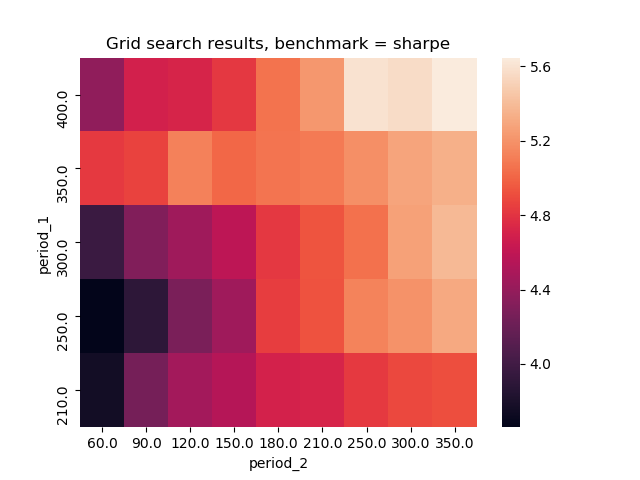
\includegraphics[width=0.6\textwidth]{GridSearches/Average_Drawdown/Figure_1.png}
	\captionof{figure}{GridSearch for the window of Sharpe Ratio and drawdown measure}
	\label{Average_Drawdown_1}
\end{center}

\begin{center}
	\centering
	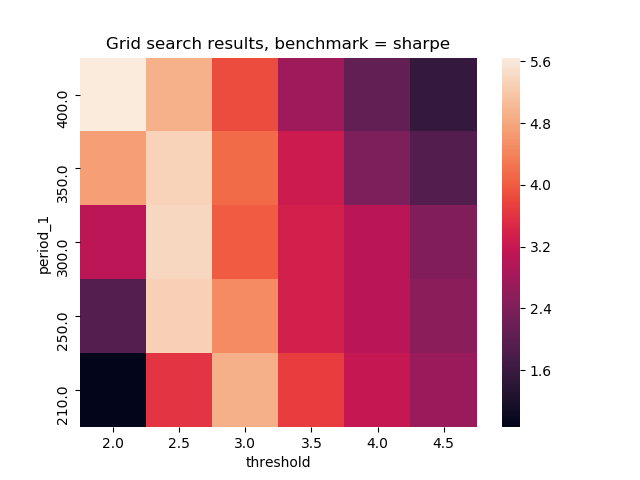
\includegraphics[width=0.6\textwidth]{GridSearches/Average_Drawdown/Figure_2.png}
	\captionof{figure}{GridSearch for the parameters relative to the Sharpe Ratio}
	\label{Average_Drawdown_2}
\end{center}

\begin{center}
	\centering
	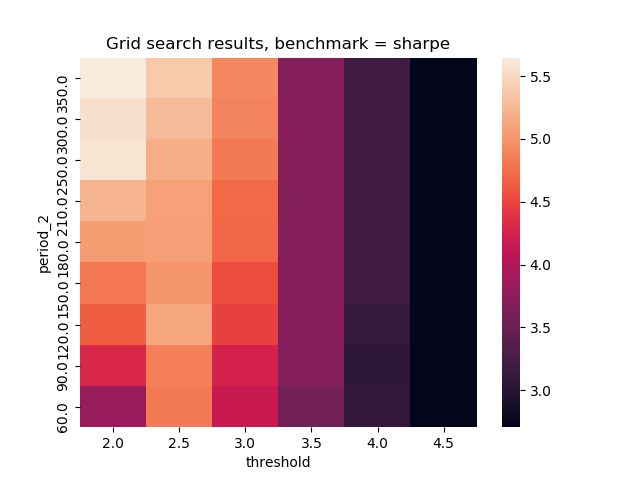
\includegraphics[width=0.6\textwidth]{GridSearches/Average_Drawdown/Figure_3.png}
	\captionof{figure}{GridSearch for drawdown window and sharpe threshold}
	\label{Average_Drawdown_3}
\end{center}
